% ULA-GesFormer IROS draft
%
% NOTE TO AUTHOR (remove this comment block before submission):
%  - Architecture renamed from the earlier "ULA-MMDiT" working name to
%    "ULA-GesFormer" per author decision: the model is a single-stream
%    conditional flow-matching transformer, not a dual-stream
%    cross-attention MM-DiT, and the new name avoids that implication.
%  - Primary target action space is now 18-DoF (waist 3 + arms 12 +
%    head 3), per author decision. The 15-DoF waist+arm subspace is the
%    only part with complete held-out evaluation, cross-domain
%    adaptation, real-time, and safety numbers; the head-DoF extension
%    is reported honestly as in-progress (Sec.~\ref{sec:head-status}).
%    Do not backfill 18-DoF "final" numbers without a real completed,
%    supervised training run -- see that section for why the existing
%    beat2_18d_from_scratch_formal_v1 run is NOT cited as a finished
%    result (behavior/emotion supervision counts are 0 in its own
%    provenance record as of 2026-07-25).
%  - This uses the portable \documentclass[conference]{IEEEtran}, which ships
%    with every standard TeX distribution and compiles as-is on Overleaf.
%    Before final submission, download the current-year official IROS
%    LaTeX template from the IROS website / Overleaf gallery and drop this
%    body content into their root.tex (their \documentclass line and any
%    required style files take precedence over this one).
%  - Fill in \author{} with real names/affiliations before sharing outside
%    the team; a placeholder is used below.
%  - Every number in this draft is taken from files in the repository
%    (see inline \todo{} notes for anything that still needs a second
%    source or a decision from you). Nothing quantitative is invented.
%  - The biggest open gap for review-readiness: there is currently no
%    head-to-head comparison against a baseline generator (e.g. an
%    unconditional or coarser-conditioned ablation). Section
%    \ref{sec:limitations} flags this explicitly -- IROS reviewers will
%    very likely ask for it, so treat it as the top priority before
%    submission, not an optional polish item.

\documentclass[conference]{IEEEtran}
\IEEEoverridecommandlockouts
\usepackage{cite}
\usepackage{amsmath,amssymb,amsfonts}
\usepackage{graphicx}
\usepackage{textcomp}
\usepackage{xcolor}
\usepackage{booktabs}
\usepackage{array}
\usepackage{tikz}
\usetikzlibrary{arrows.meta,positioning,fit,matrix,calc}
\usepackage{algorithm}
\usepackage{algpseudocode}

\newcommand{\todo}[1]{\textcolor{red}{[TODO: #1]}}

\def\BibTeX{{\rm B\kern-.05em{\sc i\kern-.025em b}\kern-.08em
    T\kern-.1667em\lower.7ex\hbox{E}\kern-.125emX}}

\begin{document}

\title{ULA-GesFormer: Emotion- and Intent-Conditioned Flow Matching \\
for Real-Time Expressive Upper-Body Gesture Generation \\
on a Social Humanoid Robot}

\author{\IEEEauthorblockN{\todo{Author Name(s)}}
\IEEEauthorblockA{\todo{Department / Lab, Institution}\\
\todo{City, Country}\\
\todo{email@institution.edu}}}

\maketitle

\begin{abstract}
Social and companion humanoid robots increasingly need to express
intent-appropriate, emotionally legible upper-body gestures in real time,
under hard joint-limit and velocity constraints that do not apply to
virtual avatars. We present ULA-GesFormer, a conditional flow-matching
transformer that generates robot upper-body joint trajectories directly,
conditioned on a structured 264-dimensional vector that fuses discrete
behavior/emotion/family labels, continuous data-driven style controls,
and a leakage-free motion-prototype descriptor. The target action space
is 18 DoF (3-DoF waist, 6-DoF per arm, 3-DoF head); the fully validated
core of the system is a 12.4M-parameter, 15-DoF (waist+arm) generator,
with an append-only 3-DoF head extension (12.40M parameters total)
under active development. The 15-DoF core is trained on a 162-class
(27 behaviors $\times$ 6 emotions) expressive-behavior dataset of
1{,}620 clips (2.25\,h) and deployed behind a text-instruction front end
and a kinematic safety filter. We show that (i) held-out reconstruction
error is essentially unchanged whether the model is driven by free-text
instructions through a semantic adapter or by direct structured labels,
(ii) the same generator, extended to 18 DoF, adapts to a public
affective conversational-gesture corpus (BEAT2) under a strict
speaker-disjoint split, reducing held-out validation and test loss by
36.0\% and 51.9\% respectively without degrading performance on the
original distribution, (iii) the full text-to-trajectory pipeline runs
at 46--67$\times$ real time on a single consumer GPU (65\,ms median
end-to-end latency for a 3\,s clip), and (iv) a kinematic safety filter
reduces raw joint- and velocity-limit violations from 1--2\% of frames
to zero while an independent blind human review found zero
self-collision frames across 29 reviewed clips. We additionally report
an exploratory LoRA-aligned Qwen text-motion latent space evaluated by
retrieval (top-1 recall 21--25\%), and we report all of this
transparently alongside open problems -- most notably the lack of a
baseline comparison, unresolved head-motion jitter in the 18-DoF
extension, and the absence of perceptual user studies -- that we
identify as the immediate next steps.
\end{abstract}

\begin{IEEEkeywords}
gesture generation, flow matching, affective human-robot interaction, humanoid robots, motion synthesis
\end{IEEEkeywords}

\section{Introduction}
\label{sec:intro}

Companion and service humanoid robots are increasingly expected to do
more than execute task motions: they must greet, comfort, refuse,
celebrate, and otherwise communicate intent and affect through
upper-body gesture, often in direct response to a natural-language
instruction or an inferred emotional state. This differs from the
well-studied problem of co-speech gesture synthesis for virtual avatars
in two important ways. First, the output is not a free SMPL-X mesh but a
fixed set of physical joints with hard position and velocity limits, so
generation error that would be imperceptible on an avatar can become an
unsafe or physically infeasible command on hardware. Second, an
interactive robot cannot tolerate multi-second generation latency: a
user who greets the robot expects a gesture to begin almost immediately.

We target an 18 degree-of-freedom (DoF) upper-body configuration
(3-DoF waist, 6-DoF per arm including wrist roll/pitch, 3-DoF head) on
a social humanoid platform, and address a companion-robot behavior
taxonomy of 27 discrete behaviors (idle, greeting, farewell, comfort,
alert, withdrawal, dance, and attention/search/error families) crossed
with 6 emotion categories (neutral, sad, happy, angry, surprise, fear),
yielding 162 semantic classes that a generator must produce
recognizably and safely, ideally from either a structured label or a
free-text instruction. The action space is designed to be extended
append-only: a 15-DoF waist+arm core (no head) is fully trained and
evaluated, and a 3-DoF head slice is added on top of it without
changing the existing joint ordering, condition scheme, or losses. We
report the 15-DoF core as the validated result of this paper and the
18-DoF head extension as an actively developed, not yet fully
converged component (Section~\ref{sec:head-status}), rather than
presenting a completed 18-DoF system that does not yet exist.

We present \textbf{ULA-GesFormer}, a compact conditional flow-matching
transformer that predicts a velocity field over the joint-trajectory
space directly, integrated with an Euler ODE sampler at inference time.
Our contributions are:

\begin{enumerate}
\item A structured 264-dimensional condition representation that
  separately projects legacy semantic/text features, discrete
  behavior/emotion/family labels, three data-derived continuous style
  scalars, and a 128-dimensional, leakage-free motion-prototype
  descriptor into seven condition tokens, so the transformer receives
  disentangled semantic evidence rather than having to discover field
  boundaries inside a single flat vector.
\item A multi-task training objective -- flow matching plus position,
  velocity, acceleration, kinematic-descriptor, motion-latent, and
  duration losses -- that lets a 12.4M-parameter, single-stream
  transformer (6 layers, 8 heads, 384 hidden dim) trained on a modest
  1{,}620-clip dataset produce smooth, duration-aware trajectories
  without a separate duration or transition model, and an append-only
  adaptation recipe that extends the same backbone to a 3-DoF head slice.
\item An exploratory shared text-motion latent space, obtained by
  LoRA-tuning a frozen Qwen3-Embedding-0.6B text encoder against a
  frozen motion-metric encoder with bidirectional retrieval and
  anti-collapse regularization, evaluated by held-out retrieval and
  representation-collapse diagnostics rather than assumed to work.
\item An evaluation spanning held-out reconstruction quality, strict
  speaker-disjoint cross-domain adaptation to a public affective-gesture
  corpus (BEAT2 \cite{beat2}), real-time inference throughput on
  consumer hardware, and physical/kinematic safety validation including
  an independent blind human review -- reported with explicit caveats
  about what is and is not yet demonstrated.
\end{enumerate}

We deliberately scope this paper around the generator; the
video-to-3D-pose and human-to-URDF retargeting pipeline that produced
part of the training data is treated as supporting infrastructure and
described only at the level needed to interpret the dataset in
Section~\ref{sec:dataset}.

\section{Related Work}
\label{sec:related}

\textbf{Data-driven affective and co-speech gesture generation.}
BEAT \cite{beat} and its holistic successor BEAT2/EMAGE
\cite{beat2} established large-scale, emotion- and semantics-annotated
conversational-gesture datasets and masked audio-gesture modeling.
EmotionGesture \cite{emotiongesture} and EMoG \cite{emog} condition
diffusion or transformer generators explicitly on emotion to resolve
the one-to-many mapping from speech to gesture, and add motion-smoothness
and joint-correlation objectives. ConvoFusion \cite{convofusion}
extends diffusion-based synthesis to multi-modal, multi-party
conversational settings with explicit controllability. Text2Gestures
\cite{text2gestures} and the theory-driven approach of Spitale and
Matari\'{c} \cite{affective-gestures-theory} generate emotive gestures
directly from text, parameterizing motion by shape, intensity, and
speed rather than emotion labels alone. Intentional Gesture
\cite{intentional-gesture} argues that gesture should carry
communicative intent rather than only speech rhythm, augmenting BEAT2
with intention annotations. LiveGesture \cite{livegesture} and MIBURI
\cite{miburi} target low-latency, streaming, causal gesture synthesis
with region-aware discrete motion tokenizers for real-time spoken
dialogue. All of the above generate full-body, unconstrained avatar
motion; none enforce hardware joint or velocity limits inside the
generative loop, and none report end-to-end latency budgets for a
physical platform, which is the regime we target.

\textbf{Generative motion models.} The Human Motion Diffusion Model
\cite{mdm} popularized diffusion-based human motion synthesis. Flow
matching \cite{flow-matching} reformulates generative modeling as
learning a straight-line probability path between noise and data,
enabling fewer-step, ODE-based sampling; MM-DiT \cite{mmdit} introduces
a dual-stream transformer with modality-specific weights and joint
cross-attention for conditional flow-matching image synthesis. Our
model borrows the flow-matching training objective and the
token-based conditioning idea from this line of work but deliberately
uses a simpler single-stream, self-attention-only transformer over
concatenated condition and motion tokens, rather than a dual-stream,
cross-attention architecture -- a design choice suited to a
sub-15M-parameter model with only seven condition tokens, and reflected
in the model name (\emph{GesFormer}: a gesture-generation transformer)
rather than borrowing MM-DiT's terminology for a different architecture.

\textbf{Human-to-robot expressive motion.} A substantial body of work
retargets human motion capture or video-derived 3D pose onto humanoid
or social-robot kinematic structures for expressive behavior libraries.
We rely on such a pipeline (monocular/multi-view 3D pose extraction,
torso-local-frame retargeting, and joint-limit/velocity safety
filtering) to help construct part of the cross-domain evaluation data
in Section~\ref{sec:experiments}, but the retargeting method itself is
not a contribution of this paper.

\section{Robot Platform and Action Space}
\label{sec:platform}

The target action space is an 18-dimensional joint-angle vector at each
timestep: pelvis yaw/pitch/roll (3), per-arm shoulder pitch/roll/yaw,
elbow, and wrist roll/pitch (6 per arm, 12 total), and head
roll/pitch/yaw (3). The model does not output finger or gripper joints.
Each dimension has a hardware joint limit and a shared angular-velocity
limit of 3\,rad/s enforced both during dataset construction and again
as a post-hoc inference-time safety filter (Section~\ref{sec:inference}).

The action space is built append-only, in two tiers. The \emph{core}
tier is the 15-DoF waist+arm subspace (pelvis + both arms, no head);
it is deliberately narrow enough for a sub-15M-parameter model trained
on a few thousand clips to master reliably, while covering the DoF
that carry most of the communicative signal in upper-body gesture
(torso orientation, arm shape, arm extension) \cite{intentional-gesture}.
The \emph{extension} tier adds the 3-DoF head slice on top of an
already-trained core checkpoint: the original 15 joints keep their
order, weights, and hardware limits, and only the newly added input/
output projection slices are updated by default. This paper reports
complete held-out evaluation, cross-domain adaptation, real-time, and
safety results for the 15-DoF core (Section~\ref{sec:experiments}),
and an honest, in-progress status report for the 18-DoF head extension
(Section~\ref{sec:head-status}); we do not claim a finished, validated
18-DoF system.

\section{Method}
\label{sec:method}

\subsection{Structured Condition Representation}
\label{sec:condition}

Rather than encoding semantics as a single opaque embedding, the
264-dimensional condition vector $c \in \mathbb{R}^{264}$ is partitioned
into six semantically distinct slices, each projected by its own
two-layer MLP (\texttt{Linear}$\to$\texttt{SiLU}$\to$\texttt{Linear},
hidden/output width 384) into one or more of seven 384-dimensional
condition tokens (Table~\ref{tab:condition}). Projecting each field
independently lets the transformer receive tokens that are already
labeled by role (``this is behavior,'' ``this is emotion,'' ``this is
style'') instead of requiring a shared encoder to rediscover field
boundaries inside a flat vector.

\begin{table}[t]
\centering
\caption{Structured 264-dimensional condition vector.}
\label{tab:condition}
\begin{tabular}{@{}lrrl@{}}
\toprule
Slice & Dim. & Tokens & Content \\
\midrule
Legacy semantic/text & 92 & 1 & intent, affect, gesture, style \\
 & & & one-hots + continuous + text feats. \\
Behavior & 27 & 1 & one-hot over Kimodo behaviors \\
Emotion & 6 & 1 & one-hot over 6 emotion classes \\
Behavior family & 8 & 1 & one-hot over 8 behavior families \\
Style controls & 3 & 1 & arm balance, amplitude, speed \\
Motion prototype & 128 & 2 & behavior$\times$emotion group mean \\
\midrule
Total & 264 & 7 & \\
\bottomrule
\end{tabular}
\end{table}

The three style controls are computed directly from motion, not
annotated: signed left/right arm-activity balance, log-amplitude, and
log-speed of the two arms, each standardized on training-split
statistics only and clipped to $[-5,5]$. At inference time these can be
sampled from a per-(behavior, emotion) style bank built from training
data, fixed at the split mean, or set explicitly.

The 128-dimensional motion-prototype slice is the mean, L2-renormalized
output of a frozen motion-metric encoder over all training clips
sharing a (behavior, emotion) pair; validation and test clips never
contribute to a prototype, which both prevents leakage and lets a
deployed generator look up a cached prototype table without re-running
the metric encoder.

\subsection{ULA-GesFormer Transformer}

Given a noised action sequence $x_t \in \mathbb{R}^{T\times D}$ ($D=15$
for the core tier, $D=18$ once the head extension is applied), a flow
time $t\in[0,1]$, and condition $c$, each of the $T$ per-frame action
vectors is linearly projected to 384 dimensions and summed with a
parameter-free sinusoidal flow-time embedding and a parameter-free
sinusoidal frame-position embedding. The resulting $T$ motion tokens are
concatenated with the 7 condition tokens from
Section~\ref{sec:condition} into a single sequence of length $T+7$ and
passed through 6 pre-LN \texttt{TransformerEncoder} layers (8 heads, 48
dim/head, 1536-dim GELU feed-forward, dropout 0.1), with unrestricted
bidirectional self-attention -- every motion frame can attend to every
condition token and every other frame. After the final layer, the 7
condition positions are discarded and the remaining $T$ positions are
mapped by \texttt{LayerNorm} $\to$ \texttt{Linear}(384,$D$) to a
predicted velocity field $v_\theta(x_t,t,c)\in\mathbb{R}^{T\times D}$.
The 15-DoF core model has 12{,}394{,}004 parameters, 85.9\% of which are
in the transformer backbone (Table~\ref{tab:params}); the append-only
18-DoF head extension adds a small number of new input/output weights
for a total of 12{,}396{,}311 parameters, all of which are trainable
once the head slice is post-trained end-to-end.

Figure~\ref{fig:arch} summarizes the two token streams and their
merge into a single bidirectional encoder. The condition stream (top)
turns the 264-D structured vector of Section~\ref{sec:condition} into
7 fixed condition tokens; the action stream (bottom) linearly embeds
the noised sequence into $T$ motion tokens carrying flow-time and
frame-position information. Both streams are concatenated -- there is
no cross-attention block and no separate condition/action towers --
and processed jointly by the shared encoder, after which the condition
positions are dropped and the motion positions are decoded into the
predicted velocity field. The duration planner reads the condition
vector directly, in parallel with the encoder, since clip length must
be known before the motion-token sequence can be constructed.

\begin{figure}[t]
\centering
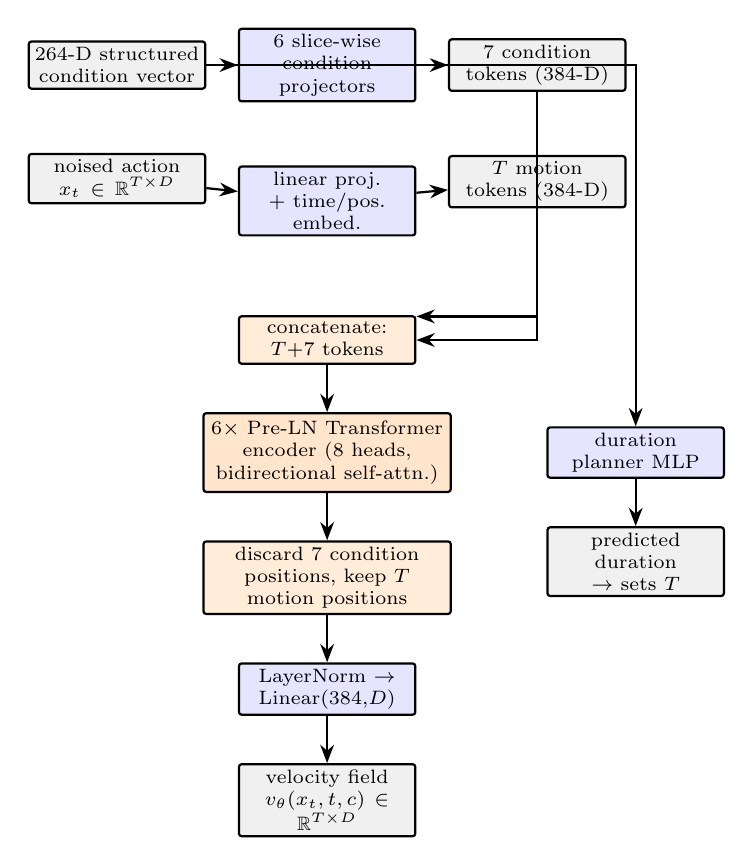
\begin{tikzpicture}[
  node distance=4mm and 4mm,
  every node/.style={font=\scriptsize},
  box/.style={draw, rounded corners=1pt, align=center, minimum height=6mm,
    inner sep=2pt, text width=2.1cm},
  >=Stealth, thick
]
\node[box, fill=gray!12] (cond) {264-D structured condition vector};
\node[box, fill=blue!10, right=of cond] (condproj) {6 slice-wise condition projectors};
\node[box, fill=gray!12, right=of condproj] (condtok) {7 condition tokens (384-D)};

\node[box, fill=gray!12, below=8mm of cond] (xt) {noised action $x_t\in\mathbb R^{T\times D}$};
\node[box, fill=blue!10, below=8mm of condproj] (aproj) {linear proj.\ + time/pos.\ embed.};
\node[box, fill=gray!12, below=8mm of condtok] (mtok) {$T$ motion tokens (384-D)};

\node[box, fill=orange!15, below=10mm of aproj] (concat) {concatenate: $T{+}7$ tokens};
\node[box, fill=orange!20, below=6mm of concat, text width=3.0cm, minimum height=10mm] (encoder) {6$\times$ Pre-LN Transformer encoder (8 heads, bidirectional self-attn.)};
\node[box, fill=orange!15, below=6mm of encoder, text width=3.0cm] (drop) {discard 7 condition positions, keep $T$ motion positions};
\node[box, fill=blue!10, below=6mm of drop] (outproj) {LayerNorm $\to$ Linear(384,$D$)};
\node[box, fill=gray!12, below=6mm of outproj] (vel) {velocity field $v_\theta(x_t,t,c)\in\mathbb R^{T\times D}$};

\node[box, fill=blue!10, right=12mm of encoder] (planner) {duration planner MLP};
\node[box, fill=gray!12, below=6mm of planner] (dur) {predicted duration $\to$ sets $T$};

\draw[->] (cond) -- (condproj);
\draw[->] (condproj) -- (condtok);
\draw[->] (xt) -- (aproj);
\draw[->] (aproj) -- (mtok);
\draw[->] (condtok.south) |- (concat.east);
\draw[->] (mtok.south) |- ($(concat.east)+(0,3mm)$);
\draw[->] (concat) -- (encoder);
\draw[->] (encoder) -- (drop);
\draw[->] (drop) -- (outproj);
\draw[->] (outproj) -- (vel);
\draw[->] (cond.east) -| ($(planner.north)+(0,3mm)$) -- (planner.north);
\draw[->] (planner) -- (dur);
\end{tikzpicture}
\caption{ULA-GesFormer architecture. The 264-D structured condition
(Section~\ref{sec:condition}) is split into six semantic slices and
projected into 7 condition tokens; the noised action sequence is
linearly embedded into $T$ motion tokens carrying flow-time and
frame-position information. Both token sets are concatenated and
processed by 6 bidirectional Pre-LN transformer encoder layers; the
condition positions are then discarded and the remaining $T$ positions
are decoded into a per-frame velocity field. A separate MLP reads the
same condition vector, in parallel, to predict clip duration.}
\label{fig:arch}
\end{figure}

\begin{table}[t]
\centering
\caption{Parameter breakdown of the 15-DoF core generator.}
\label{tab:params}
\begin{tabular}{@{}lr@{}}
\toprule
Module & Parameters \\
\midrule
Transformer backbone (6 layers) & 10{,}646{,}784 \\
Six condition projectors & 1{,}483{,}008 \\
Action input projection & 6{,}144 \\
Output LayerNorm + projection & 6{,}543 \\
Duration planner MLP & 249{,}600 \\
Duration head & 385 \\
Transition head (unsupervised, see \S\ref{sec:limitations}) & 1{,}540 \\
\midrule
Total & 12{,}394{,}004 \\
\bottomrule
\end{tabular}
\end{table}

A separate planner MLP (\texttt{Linear}(264,384)$\to$\texttt{SiLU}
$\to$\texttt{Linear}(384,384)$\to$\texttt{SiLU}$\to$\texttt{Linear}
(384,1)$\to$\texttt{Softplus}$+0.25$) reads the same condition vector
and predicts clip duration in seconds, so a deployed generator does not
need an externally specified clip length. The architecture also defines
a 4-way transition-type head (continue / emotion change / action
change / end); this head is currently unsupervised (\S\ref{sec:limitations}).

\subsection{Training Process}
\label{sec:training}

Training uses the standard flow-matching interpolation $x_t =
(1-t)z + tx$ for $z\sim\mathcal N(0,I)$ and target velocity $v^\ast = x
- z$. The total loss is
\begin{equation}
\label{eq:loss}
\begin{aligned}
\mathcal{L} = {}& 1.0\,\mathcal{L}_{\text{flow}} + 0.25\,\mathcal{L}_{\text{pos}} + 0.01\,\mathcal{L}_{\text{vel}} \\
& + 0.0005\,\mathcal{L}_{\text{acc}} + 0.001\,\mathcal{L}_{\text{desc}} \\
& + 0.1\,\mathcal{L}_{\text{latent}} + 0.1\,\mathcal{L}_{\text{dur}},
\end{aligned}
\end{equation}
where $\mathcal{L}_{\text{flow}}$ is the MSE between predicted and
target velocity; $\mathcal{L}_{\text{pos}}$ is a Smooth-L1 loss between
the one-step endpoint estimate $\hat x = x_t + (1-t)v_\theta$ and $x$;
$\mathcal{L}_{\text{vel}}$/$\mathcal{L}_{\text{acc}}$ penalize first-
and second-order frame differences using the clip's true duration;
$\mathcal{L}_{\text{desc}}$ matches a 48-dimensional set of kinematic
descriptors (amplitude, speed, acceleration, left/right balance);
$\mathcal{L}_{\text{latent}}$ is a cosine distance in the frozen
motion-metric embedding space between generated and reference motion;
and $\mathcal{L}_{\text{dur}}$ matches $\log(1+\text{seconds})$ between
predicted and true duration.

Figure~\ref{fig:training} lays out one training iteration end to end.
Each batch of 64 clips is drawn with a balanced sampler over the 162
(behavior, emotion, style) classes of Section~\ref{sec:dataset},
stratified by left/right laterality and motion amplitude so that rare,
high-energy expressive clips are not drowned out by neutral,
low-amplitude ones. Each clip is phase-resampled to one of three
lengths ($64$, $96$, or $128$ frames) so the model sees consistent
short/medium/long phase structure rather than a single fixed duration.
The 264-D condition is built per Section~\ref{sec:condition} (with the
motion prototype looked up from the pre-computed, leakage-free table),
noise and flow time are sampled, and $x_t$ is formed as above. A
forward pass produces $v_\theta$, the loss in Eq.~\ref{eq:loss} is
computed, and gradients are backpropagated with global-norm clipping
at 1.0. Parameters are updated with AdamW (learning rate $10^{-4}$,
weight decay $10^{-4}$, linear warm-up over the first 1{,}000 steps
followed by cosine decay to $0.1\times$ the peak rate), and an
exponential moving average of the weights (decay $0.999$) is
maintained for evaluation and export. Every 500 steps, the run is
validated on the held-out split, a checkpoint is written, and (for
runs with previews enabled) a MuJoCo rollout is rendered for
qualitative inspection.

\begin{figure*}[t]
\centering
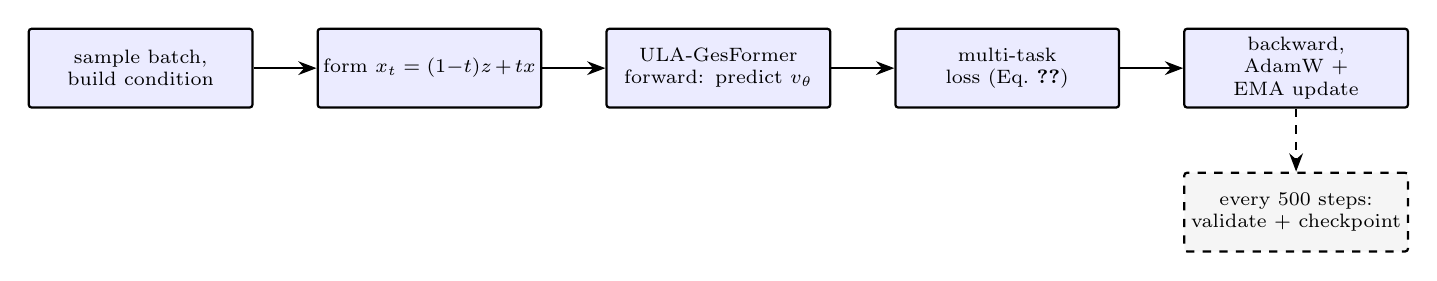
\begin{tikzpicture}[
  node distance=8mm,
  every node/.style={font=\scriptsize},
  box/.style={draw, rounded corners=1pt, align=center, fill=blue!8,
    minimum height=10mm, text width=2.7cm, inner sep=2pt},
  periodic/.style={box, dashed, fill=gray!8},
  >=Stealth, thick
]
\node[box] (batch) {sample batch,\\build condition};
\node[box, right=of batch] (noise) {form $x_t=(1{-}t)z+tx$};
\node[box, right=of noise] (fwd) {ULA-GesFormer forward: predict $v_\theta$};
\node[box, right=of fwd] (loss) {multi-task loss (Eq.~\ref{eq:loss})};
\node[box, right=of loss] (update) {backward,\\AdamW + EMA update};
\node[periodic, below=8mm of update] (val) {every 500 steps:\\validate + checkpoint};

\draw[->] (batch) -- (noise);
\draw[->] (noise) -- (fwd);
\draw[->] (fwd) -- (loss);
\draw[->] (loss) -- (update);
\draw[->, dashed] (update) -- (val);
\end{tikzpicture}
\caption{One training iteration. Batch sampling and conditioning
follow Section~\ref{sec:condition}; the forward pass is the
ULA-GesFormer model of Figure~\ref{fig:arch}; the periodic
validation/checkpoint step (dashed) runs every 500 steps, not every
iteration.}
\label{fig:training}
\end{figure*}

\subsection{Inference Process}
\label{sec:inference}

Inference starts from Gaussian noise in normalized joint space and
integrates the learned velocity field with $N$ Euler steps
($dt=1/N$), clamping to the normalized joint range after every step:
$x \leftarrow \mathrm{clamp}(x + dt\,v_\theta(x,t,c))$. Free-text
instructions are first parsed by a Qwen-based semantic adapter into a
(behavior, emotion) pair, which selects the corresponding base
condition and cached motion prototype; a style vector is drawn from the
per-class style bank; the planner predicts a duration, which sets $T$.
After integration, the trajectory is de-normalized to radians and
passed through the same joint-limit and 3\,rad/s velocity-limit filter
used during dataset construction before being sent to the robot or
simulator. Figure~\ref{fig:inference} and Algorithm~\ref{alg:inference}
give the pipeline and the sampling loop in full; unlike training, no
ground-truth clip, duration, or condition label is available, so every
quantity used at inference is either predicted by the network or drawn
from the fixed, precomputed style/prototype tables.

\begin{figure}[t]
\centering
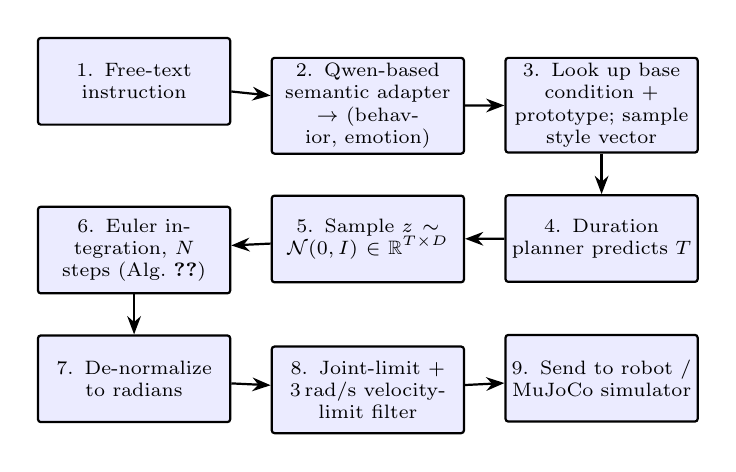
\begin{tikzpicture}[
  every node/.style={font=\scriptsize},
  box/.style={draw, rounded corners=1pt, align=center, fill=blue!8,
    minimum height=11mm, text width=2.3cm, inner sep=2pt},
  >=Stealth, thick
]
\matrix (n) [matrix of nodes, nodes=box, row sep=5mm, column sep=5mm] {
1. Free-text instruction &
2. Qwen-based semantic adapter $\to$ (behavior, emotion) &
3. Look up base condition + prototype; sample style vector \\
6. Euler integration, $N$ steps (Alg.~\ref{alg:inference}) &
5. Sample $z\sim\mathcal N(0,I)\in\mathbb R^{T\times D}$ &
4. Duration planner predicts $T$ \\
7. De-normalize to radians &
8. Joint-limit + 3\,rad/s velocity-limit filter &
9. Send to robot / MuJoCo simulator \\
};
\draw[->] (n-1-1) -- (n-1-2);
\draw[->] (n-1-2) -- (n-1-3);
\draw[->] (n-1-3) -- (n-2-3);
\draw[->] (n-2-3) -- (n-2-2);
\draw[->] (n-2-2) -- (n-2-1);
\draw[->] (n-2-1) -- (n-3-1);
\draw[->] (n-3-1) -- (n-3-2);
\draw[->] (n-3-2) -- (n-3-3);
\end{tikzpicture}
\caption{Inference pipeline. Steps 1--4 turn free text into a
condition and a predicted duration; steps 5--6 run the Euler sampler
of Algorithm~\ref{alg:inference}; steps 7--9 de-normalize, apply the
kinematic safety filter, and dispatch the trajectory.}
\label{fig:inference}
\end{figure}

\begin{algorithm}[t]
\caption{Inference-time Euler sampling}
\label{alg:inference}
\begin{algorithmic}[1]
\Require condition $c$ (behavior, emotion, style, prototype), predicted
duration $T$, step count $N$
\State $x \sim \mathcal N(0,I) \in \mathbb R^{T\times D}$ \Comment{normalized joint space}
\State $dt \leftarrow 1/N$
\For{$k = 0, \dots, N-1$}
  \State $t \leftarrow k\,dt$
  \State $v \leftarrow v_\theta(x, t, c)$ \Comment{ULA-GesFormer forward pass, Fig.~\ref{fig:arch}}
  \State $x \leftarrow x + dt\,v$
  \State $x \leftarrow \mathrm{clamp}(x, x_{\min}, x_{\max})$ \Comment{normalized joint range}
\EndFor
\State $x_{\text{rad}} \leftarrow \textsc{DeNormalize}(x)$
\State $x_{\text{rad}} \leftarrow \textsc{SafetyFilter}(x_{\text{rad}})$ \Comment{joint-limit + 3\,rad/s velocity clamp}
\State \Return $x_{\text{rad}}$
\end{algorithmic}
\end{algorithm}

\subsection{Qwen Text-Motion Latent Alignment (Exploratory)}
\label{sec:qwen-latent}

The deployed pipeline above uses a classification-based semantic
adapter: text is mapped to a discrete (behavior, emotion) pair, which
looks up a fixed condition. In parallel, we train a differentiable
\emph{shared latent space} between free-form text and motion, intended
as a future retrieval- or embedding-conditioned alternative rather than
a replacement for the deployed path. A frozen Qwen3-Embedding-0.6B
encoder is adapted with a rank-8 LoRA (top 4 layers, $q,k,v,o$
projections) and a text projection head into a normalized
128-dimensional text latent; a frozen motion-metric encoder (the same
one used for the motion-prototype descriptor and $\mathcal L_{\text{latent}}$
in Section~\ref{sec:condition}) produces the corresponding 128-dimensional
motion latent for a 150-frame trajectory. Training combines
bidirectional text-motion retrieval, text behavior/emotion
classification, teacher anchoring to the original frozen motion
encoder, and VICReg variance/covariance regularization to discourage
representation collapse, on a split of 1{,}296 training episodes with
810 text prompts and 162 validation/162 test episodes with disjoint
paraphrases.

At 100{,}000 steps, held-out validation retrieval reaches
text-to-motion Recall@1 21.0\% / Recall@5 51.9\% and motion-to-text
Recall@1 24.7\% / Recall@5 50.0\% (median rank 5 of 162); text-side
auxiliary classification is strong (behavior accuracy 93.2\%, emotion
accuracy 96.3\%) but motion-side classification from the aligned latent
is weaker (behavior 45.8\%, emotion 66.7\%), and the motion latent's
effective rank (19.6 of 128) is substantially lower than the text
latent's (45.7 of 128), indicating the motion embedding is more
collapsed than the text embedding at this training point. We report
these numbers as a diagnostic of an exploratory representation-learning
track, not as a generation-quality result: per the component's own
design scope, this latent space \emph{does not yet feed the deployed
264-dimensional condition contract}, and a generator would still need
to be trained or adapted to consume it before any deployment claim
could be made.

\section{Dataset}
\label{sec:dataset}

\textbf{Kimodo (primary training set).} Kimodo is an expressive-behavior
taxonomy for the target social-robot platform: 27 behaviors (idle,
greeting/farewell, comfort, alert, withdrawal, dance, and
attention/search/error variants) crossed with 6 emotion categories
(neutral, sad, happy, angry, surprise, fear), giving 162 semantic
classes. The exported training set contains 1{,}620 episodes
(10 per class), 243{,}000 frames at 30\,fps (2.25\,h total), split
1{,}296/162/162 into train/validation/test while preserving class
balance. A training-time sampler rotates uniformly across the 162
classes and, with probability 0.5, further stratifies by
laterality/amplitude bucket so that common labels or common motion
amplitudes do not dominate training.

\textbf{BEAT2 (cross-domain adaptation set).} To evaluate generalization
beyond Kimodo's authored behaviors, we retarget a subset of the public
BEAT2 conversational-gesture corpus \cite{beat2} (5 speakers, Chinese)
to an 18-DoF variant of the robot joint space (adding head yaw/pitch/roll
to the 15-DoF base) and evaluate under a strict, speaker-disjoint split:
4{,}570 candidate 6\,s windows are quality-checked, of which 3{,}495
pass (76.5\% pass rate, 6.27\,h, 677{,}092 frames). Training uses
speakers 13\_lu, 22\_luqi, and 23\_hailing (2{,}026 records); validation
uses speaker 12\_zhao (1{,}125 records); test uses speaker 24\_kexin,
held out entirely (344 records). No speaker appears in more than one
split. This is the dataset used for the 18-DoF post-training experiment
in Section~\ref{sec:beat2-adapt} and the real-time benchmark in
Section~\ref{sec:realtime}.

\textbf{Large-scale motion-only pretraining pool (18-DoF, in
progress).} Separately from the supervised BEAT2 subset above, we are
scaling 18-DoF pretraining to a much larger BEAT2 pool (12{,}345
episodes: 9{,}712 train / 1{,}384 validation / 1{,}249 test) that has
passed motion-quality QC but, as of this writing, carries \emph{no}
supervised behavior or emotion labels -- every episode's behavior and
emotion fields are recorded as unresolved/candidate in the dataset's
own provenance record. We report this honestly as a motion-only
pretraining pool intended to precede supervised behavior/emotion
fine-tuning, not as an emotion-conditioned training set, and we do not
report generation-quality numbers from it in this paper
(Section~\ref{sec:head-status}).

\section{Experiments}
\label{sec:experiments}

\subsection{Held-Out Reconstruction Quality on Kimodo (15-DoF Core)}
\label{sec:heldout}

We compare two condition sources on the same 162-class held-out test
split (162 clips), best-of-1 sampling, seed 7, 32 Euler steps: (i)
\emph{general}, which conditions directly on the structured
(behavior, emotion) label, and (ii) \emph{LoRA}, which conditions on
the same label routed through a text instruction and a LoRA-adapted
text encoder, exercising the full instruction-to-trajectory path a
user-facing deployment would use. We also evaluate both variants on
Chinese paraphrases of the same instructions to test robustness to
surface-form text variation.

\begin{table}[t]
\centering
\caption{Held-out test-set trajectory error (Kimodo, best-of-1, seed 7, 32 steps). Lower is better.}
\label{tab:heldout}
\begin{tabular}{@{}lrrr@{}}
\toprule
Variant & Pos. RMSE & Vel. RMSE & Range RMSE \\
 & (rad) & (rad/s) & (rad) \\
\midrule
General (label-conditioned) & 0.289 & 0.976 & -- \\
LoRA (text-conditioned) & 0.292 & 0.982 & 0.260 \\
LoRA (zh paraphrase) & 0.301 & 0.977 & -- \\
General (zh paraphrase) & 0.289 & 0.976 & -- \\
\bottomrule
\end{tabular}
\end{table}

Text-conditioned generation is within 1--4\% of direct-label
conditioning on every metric (Table~\ref{tab:heldout}), and is stable
under paraphrasing, indicating that the semantic adapter does not
introduce meaningful degradation versus giving the generator the
ground-truth label directly. As expected, the label-conditioned variant
is exactly invariant to paraphrasing (it never sees the raw text), and
should not be read as a stronger result -- it is not exercising a text
path at all.

\subsection{Cross-Domain Adaptation to BEAT2}
\label{sec:beat2-adapt}

We post-train the 18-DoF variant of the generator for 2{,}000 steps on
the BEAT2 training split described in Section~\ref{sec:dataset}.
Held-out validation loss drops from 5.997 to 3.840 (36.0\% reduction)
and held-out test loss (on the entirely unseen speaker 24\_kexin) drops
from 7.786 to 3.743 (51.9\% reduction). To check for catastrophic
forgetting of the original Kimodo distribution, we track loss on a
fixed Kimodo replay set before and after post-training: 0.2903 to
0.2998, a delta of 0.0095, below the pre-registered tolerance of 0.02.
On a small, single-seed diagnostic sample (3 held-out clips, matched
condition and seed before/after), position RMSE improves by 20.2\% and
velocity RMSE worsens by 5.4\%; we report this only as a diagnostic
signal, not as a primary result, since the sample is too small to
support a statistical claim (\S\ref{sec:limitations}).

\subsection{Real-Time Inference}
\label{sec:realtime}

We benchmark the full text-to-trajectory pipeline (Qwen semantic
adapter $+$ generator, models resident, warm) on a single NVIDIA
RTX~5090 GPU, generating a 90-frame (3\,s at 30\,Hz) clip with 24
Euler steps. Median latency is 19.6\,ms for text encoding and 45.5\,ms
for trajectory generation, 65.0\,ms end-to-end -- a $46.2\times$
real-time factor relative to 30\,Hz playback. Generator-only forward
throughput (excluding text encoding) reaches 533.7 calls/s and
2{,}001.3 output frames/s, i.e. a $66.7\times$ real-time factor,
showing headroom for larger sampling budgets or model capacity while
remaining interactive.

\subsection{Safety and Physical Validation}
\label{sec:safety}

Across an audited batch of 195 clips that passed retargeting quality
control, the safety filter reduces raw joint-limit and velocity-limit
violation rates of 1.6\% and 1.3\% of frames (pre-filter) to 0\% of
frames (post-filter) by construction, and self-collision frame rate is
0.0\% for every audited clip. In an independent blind human review
protocol (three-tier affect adjudication) applied to 29 generated
clips, 24/29 were accepted as semantic-conditioning training-ready and
0/29 exhibited any self-collision frame under a 0.05 frame-rate
threshold.

\subsection{18-DoF Head Extension: Current Status}
\label{sec:head-status}

Because the 18-DoF head extension is our primary target action space
but is not yet a finished result, we report its status directly rather
than only in a limitations paragraph. Two efforts are in progress.
First, the 2{,}000-step BEAT2 post-training run used elsewhere in this
section (Sections~\ref{sec:beat2-adapt}--\ref{sec:realtime}) already trains the full
18-DoF model, but a separate, dedicated audit of generated-vs-reference
head motion on that checkpoint found substantially amplified jitter:
velocity, acceleration, and jerk RMS ratios of roughly $14\times$,
$88\times$, and $273\times$ the reference motion, respectively, with
essentially no improvement from post-training itself (all three ratios
changed by less than 0.4\% relative to the pre-post-training checkpoint).
Simple offline low-pass filtering reduces jerk substantially but at the
cost of 40--50\% of head amplitude range, which we treat as a temporary
mitigation, not a fix. Second, we are pretraining the same architecture
on the larger, motion-only 18-DoF BEAT2 pool described in
Section~\ref{sec:dataset} as a precursor to supervised behavior/emotion
fine-tuning; that run is ongoing at the time of writing and we
deliberately do not report its loss curves as a finished result, since
its own provenance record shows zero supervised behavior/emotion
labels in the current pool. We view head-motion smoothness as an open
modeling problem -- likely requiring stronger temporal-smoothness
supervision on that specific DoF group, given that the waist and arm
DoFs in the same architecture do not exhibit this failure mode -- and
we plan to report a completed, supervised 18-DoF result, including a
repeat of the full evaluation protocol in
Sections~\ref{sec:heldout}--\ref{sec:safety}, once it converges.

\section{Limitations and Future Work}
\label{sec:limitations}

We report the following limitations explicitly rather than deferring
them to a "future work" afterthought, since several bear directly on
how the above results should be read.

\textbf{No baseline comparison yet.} All reconstruction and
adaptation numbers in Section~\ref{sec:experiments} are reported
against reference motion, not against an alternative generator (e.g.\
an unconditional model, a coarser-label-only ablation, or a prior
architecture). \todo{Add at least one baseline (e.g.\ label-only vs.\
full 264-D condition, or a diffusion baseline) before submission --
reviewers will very likely request this.}

\textbf{Single-seed diagnostic metrics.} The trajectory-level RMSE
numbers reported for BEAT2 adaptation (\S\ref{sec:beat2-adapt}) come
from three clips at one seed and are explicitly diagnostic; the
held-out loss reduction is the primary, statistically meaningful
result for that experiment. \todo{Consider expanding the diagnostic
sample or dropping it in favor of the aggregate loss numbers only.}

\textbf{No perceptual or user study.} We have not yet collected
Likert-style or preference-based human ratings of generated motion
quality, emotion recognizability, or safety perception; the human
review reported in \S\ref{sec:safety} is a categorical,
expert-adjudicated accept/reject protocol over training-data
candidates, not a study of generator output quality with naive
participants. \todo{A perceptual user study (e.g.\ emotion-recognition
accuracy, preference vs.\ baseline) is likely necessary for a strong
IROS submission.}

\textbf{Unsupervised transition head.} The 4-way transition-type head
is defined in the architecture but receives no gradient under the
current V2 training objective; its outputs should not be treated as a
trained prediction.

\textbf{18-DoF extension is the primary target but is not yet a
finished, supervised result.} As detailed in
Section~\ref{sec:head-status}, the head-DoF slice currently exhibits
substantially amplified jitter relative to reference motion, and the
larger-scale pretraining pool intended to precede a full supervised
18-DoF run currently lacks behavior/emotion supervision. Every
quantitative claim in this paper that requires supervised behavior/
emotion conditioning (Section~\ref{sec:heldout}) is therefore
reported on the 15-DoF core only; results that involve the 18-DoF
checkpoint (Sections~\ref{sec:beat2-adapt}--\ref{sec:realtime}) are reported as such
and should not be read as evidence that the head extension itself is
solved.

\section{Conclusion}

We presented ULA-GesFormer, a compact conditional flow-matching
transformer that generates safety-filtered, real-time upper-body
gestures for a social humanoid robot from either structured
emotion/behavior labels or free-text instructions. Its 15-DoF
waist+arm core is fully evaluated: held-out reconstruction is stable
across text and label conditioning, the same generator adapts to a
public affective-gesture corpus under a strict speaker-disjoint split
without degrading on its original training distribution, the full
pipeline runs tens of times faster than real time on a single consumer
GPU, and a kinematic safety filter combined with independent blind
human review shows zero collision frames across all audited clips. Our
primary target, an 18-DoF extension that adds head motion and an
exploratory Qwen-aligned text-motion latent space, is reported
honestly as work in progress rather than a finished result. We view
this as a system-level starting point: the most important next steps
are completing supervised 18-DoF training with resolved head-jitter
behavior, a controlled baseline comparison, and a perceptual human
study of generated gesture quality, all of which we have scoped as
immediate future work.

\bibliographystyle{IEEEtran}
\begin{thebibliography}{00}

\bibitem{beat}
H. Liu, Z. Zhu, N. Iwamoto, Y. Peng, Z. Li, Y. Zhou, E. Bozkurt, and B. Zheng,
``BEAT: A large-scale semantic and emotional multi-modal dataset for conversational gestures synthesis,''
\emph{arXiv preprint arXiv:2203.05297}, 2022.

\bibitem{beat2}
H. Liu, Z. Zhu, G. Becherini, Y. Peng, M. Su, Y. Zhou, X. Zhe, N. Iwamoto, B. Zheng, and M. J. Black,
``EMAGE: Towards unified holistic co-speech gesture generation via expressive masked audio gesture modeling,''
\emph{arXiv preprint arXiv:2401.00374}, 2024.

\bibitem{emotiongesture}
X. Qi, C. Liu, L. Li, J. Hou, H. Xin, and X. Yu,
``EmotionGesture: Audio-driven diverse emotional co-speech 3D gesture generation,''
\emph{arXiv preprint arXiv:2305.18891}, 2023.

\bibitem{emog}
L. Yin, Y. Wang, T. He, J. Liu, W. Zhao, B. Li, X. Jin, and J. Lin,
``EMoG: Synthesizing emotive co-speech 3D gesture with diffusion model,''
\emph{arXiv preprint arXiv:2306.11496}, 2023.

\bibitem{convofusion}
M. H. Mughal, R. Dabral, I. Habibie, L. Donatelli, M. Habermann, and C. Theobalt,
``ConvoFusion: Multi-modal conversational diffusion for co-speech gesture synthesis,''
\emph{arXiv preprint arXiv:2403.17936}, 2024.

\bibitem{text2gestures}
U. Bhattacharya, N. Rewkowski, A. Banerjee, P. Guhan, A. Bera, and D. Manocha,
``Text2Gestures: A transformer-based network for generating emotive body gestures for virtual agents,''
\emph{arXiv preprint arXiv:2101.11101}, 2021.

\bibitem{affective-gestures-theory}
M. Spitale and M. J. Matari\'{c},
``Toward automated generation of affective gestures from text: A theory-driven approach,''
\emph{arXiv preprint arXiv:2103.03079}, 2021.

\bibitem{intentional-gesture}
P. Liu, H. Liu, L. Song, J. J. Corso, and C. Xu,
``Intentional gesture: Deliver your intentions with gestures for speech,''
\emph{arXiv preprint arXiv:2505.15197}, 2025.

\bibitem{livegesture}
M. U. Saleem, M. J. Patel, E. Pinyoanuntapong, Z. Qin, L. Yang, H. Xue, A. Helmy, C. Chen, and P. Wang,
``LiveGesture: Streamable co-speech gesture generation model,''
\emph{arXiv preprint arXiv:2604.10927}, 2026.

\bibitem{miburi}
M. H. Mughal, R. Dabral, V. Demberg, and C. Theobalt,
``MIBURI: Towards expressive interactive gesture synthesis,''
\emph{arXiv preprint arXiv:2603.03282}, 2026.

\bibitem{mdm}
G. Tevet, S. Raab, B. Gordon, Y. Shafir, D. Cohen-Or, and A. H. Bermano,
``Human motion diffusion model,''
\emph{arXiv preprint arXiv:2209.14916}, 2022.

\bibitem{flow-matching}
Y. Lipman, R. T. Q. Chen, H. Ben-Hamu, M. Nickel, and M. Le,
``Flow matching for generative modeling,''
\emph{arXiv preprint arXiv:2210.02747}, 2022.

\bibitem{mmdit}
P. Esser, S. Kulal, A. Blattmann, R. Entezari, J. M\"{u}ller, H. Saini, Y. Levi, D. Lorenz, A. Sauer, F. Boesel, D. Podell, T. Dockhorn, Z. English, K. Lacey, A. Goodwin, Y. Marek, and R. Rombach,
``Scaling rectified flow transformers for high-resolution image synthesis,''
\emph{arXiv preprint arXiv:2403.03206}, 2024.

\end{thebibliography}

\end{document}
